\documentclass[../../main.tex]{subfiles}
% \graphicspath{{\subfix{../images/}}}

\begin{document}
Los programas y las políticas públicas de desarrollo suelen estar diseñados para cambiar
resultados, como aumentar los ingresos, mejorar el aprendizaje o reducir las enfermedades
\cite{gertler-2016}. Saber si estos cambios se logran o no es una pregunta crucial para
quienes diseñan e implementan dichos programas, y el método para responderla es lo que se
conoce como \textbf{evaluación de impacto}.

Una evaluación de impacto mide los cambios en el bienestar de los individuos que se pueden
atribuir a un proyecto, un programa o una política específicos \cite{gertler-2016}. Su
sello distintivo es que pueden proporcionar \textbf{evidencia} robusta y creíble
sobre si un programa concreto ha alcanzado o está alcanzando sus objetivos
\cite{gertler-2016}.

Estas evaluaciones ponen un fuerte énfasis en los resultados y buscan responder una
pregunta específica de causa y efecto: ¿cuál es el impacto (o efecto causal) de un
programa? Intentan identificar y cuantificar los cambios directamente atribuibles al
tratamiento \cite{gertler-2016} sobre un conjunto de \textbf{variables de resultado} o
\textbf{de interés} en un conjunto de individuos \cite{bernal}. Estas variables son
aquellas sobre las cuales se espera que el programa tenga un efecto en los beneficiarios
\cite{bernal}. Podrían ser por ejemplo en el caso de un programa de nutrición, la estatura
y peso de los individuos; en una política de financiamento, la cantidad de empleados o de
ventas en una empresa; o en un tratamiento de acceso a medicamentos, indicadores de salud
de un paciente.

Por lo tanto, el objetivo final de la evaluación de impacto consiste en establecer lo que
se conoce como \textbf{efecto del tratamiento}, que es la diferencia entre la variable de
resultado del individuo participante en el programa en presencia del programa, y la
variable de resultado de ese individuo en ausencia del programa \cite{bernal}. Sin
embargo, es evidente que la respuesta a qué habría pasado con los beneficiarios si no
hubieran recibido el tratamiento se refiere a una situación que no es observable. Este
resultado hipotético se denomina \textbf{contrafactual} (o contrafáctico) y es lo que se
debe estimar en cualquier evaluación de impacto.

Algunas de las principales razones por las que se debería promover el uso de estas
evaluaciones como herramientas de gestión provienen del hecho que permiten mejorar la
rendición de cuentas, la inversión de recursos públicos o la efectividad de una política,
obtener financiamiento, como así también probar modalidades de programas alternativos o
innovaciones de diseño \cite{gertler-2016}.

Un ejemplo claro de por qué son necesarias las evaluaciones de impacto es el que describe
Howard White con respecto al Programa Integrado de Nutrición en Bangladesh (PINB)
\cite{white2009theory}. Este programa identificaba, mediante mediciones en campo, a los
niños desnutridos y los asignaba a un tratamiento que incluía alimentación suplementaria a
los menores y educación nutricional a las madres \cite{bernal}. Inicialmente, el programa
fue considerado como un éxito ya que los datos de monitoreo mostraban caídas importantes
en los niveles de desnutrición. El Banco Mundial decidió, con base en esta evidencia y
previo a cualquier tipo de evaluación, aumentar los recursos destinados al programa. Sin
embargo, las primeras evaluaciones de impacto, realizadas por el Grupo Independiente de
Evaluación del mismo Banco Mundial y por la ONG inglesa \textit{Save the Children},
mostraron que la mejoría de los indicadores de los beneficiarios era similar o inferior a
la de otros niños con características comparables que no hacían parte del programa
\cite{bernal}. Estos resultados reflejaron que las percepciones de los administradores del
programa y de las entidades financiadoras eran erradas, y sugirieron algunos correctivos
al programa \cite{bernal}.

Otro ejemplo que evidencia la importancia de estas evaluaciones es proporcionado por
\cite{preschool-africa-2012}, donde se evaluó el efecto de un programa de preescolar
comunitario en zonas rurales de Mozambique, lanzado en 2008 por la organización \textit{Save the
Children}. El programa consistió específicamente en el financiamiento de la construcción,
equipamiento y entrenamiento de 67 aulas en 30 comunidades \cite{preschool-africa-2012}. El
objetivo principal era verificar si un desarrollo en la infancia temprana contribuía a
preparar a los niños para la escuela y las etapas posteriores de la vida. Los resultados
mostraron no solo que la inscripción a la escuela primaria se incrementó en un 24\% en las
comunidades tratadas, sino también que los niños beneficiarios dedicaban un promedio de
7.2 horas adicionales por semana a actividades escolares y redujeron el tiempo destinado a
trabajos en las granjas familiares y a asistir a encuentros comunitarios. Además, la
participación en el programa preescolar mostró mejoras consistentes en habilidades motoras
finas, cognitivas, y de resolución de problemas \cite{preschool-africa-2012}. Todos estos
resultados contribuyeron a reforzar la idea de que los programas preescolares constituyen
una política prometedora para mejorar la preparación escolar de niños pobres y
desfavorecidos en áreas rurales de África.

Habiéndonos enfocado en el \textit{qué} es una evaluación de impacto, a continuación,
presentamos \textit{cómo} se lleva a cabo una, detallando los elementos presentes y los
problemas que pueden surgir al hacerlo.

\subsection{Estimación del Tratamiento}
Como mencionamos anteriormente, el resultado deseado al llevar a cabo una evaluación de
impacto es el efecto del tratamiento sobre un determinado indivuduo, y se obtiene como la
diferencia entre el resultado observado y el contrafáctico. Ahora bien, el marco teórico
estándar para formalizar este problema se conoce como \textbf{modelo de resultados
potenciales} o \textbf{modelo causal de Rubin} \cite{rubin1974}.

En este, se definen dos elementos para cada individuo \(i = 1,...,N\), donde \(N\)
denota la población total bajo análisis:
\begin{itemize}[itemsep=0.2cm]
    \item Por un lado, el indicador de tratamiento \(D\), tal que \(D_i = 1\) implica
    que el individuo \(i\) participó del tratamiento, y \(D_i = 0\) que no lo hizo.
    \item Por otro lado, para las variables de resultado se define \(Y_i(D_i) = (Y_i|D_i)\)
    - se lee como ``el valor de \(Y_i\) \textit{dado} \(D_i\)''. De esta forma, \(Y_i(1)\)
    es la variable de resultado si el individuo \(i\) es tratado, e \(Y_i(0)\) es la
    variable de resultado si el individuo \(i\) no es tratado. Estos valores son los
    resultados potenciales.
\end{itemize}

Con esto, el \textbf{efecto del tratamiento} para un individuo \(i\) se puede escribir como:
\begin{equation}
    \tau_i = Y_i(1) - Y_i(0) = (Y_i|D_i=1) - (Y_i|D_i=0)
    \label{eq:ite} % ite = individual treatment effect
\end{equation}

Según esta fórmula, el impacto causal (\(\tau\)) de un programa (\(D\)) en una variable de
resultado (\(Y\)) para un individuo \(i\) es la diferencia entre la variable con el
programa (\(Y_i(1)\)) y la misma variable sin el programa (\(Y_i(0)\)).

De nuevo, el problema fundamental de la evaluación de impacto es que se intenta medir una
variable en un mismo momento del tiempo para la misma unidad de observación pero en dos
realidades diferentes. Sin embargo, en la realidad, solo se observa uno de los dos resultados
potenciales \(Y_i(1)\) o \(Y_i(0)\), pero no ambos. Es decir, en los datos queda solamente
registrado \(Y_i(1)\) si \(D_i=1\) e \(Y_i(0)\) si \(D_i=0\); no se dispone de \(Y_i(1)\)
si el individuo no fue tratado (\(D_i=0\)), ni tampoco de \(Y_i(0)\) si el individuo fue
tratado (\(D_i=1\)). De esta manera, el \textbf{resultado observado de \(Y_i\)} se puede
expresar como:
\begin{equation}
    Y_i = D_i Y_i(1) + (1-D_i)Y_i(0) =
    \begin{cases}
        Y_i(1) \text{ si } D_i=1 \\
        Y_i(0) \text{ si } D_i=0
    \end{cases}
    \label{eq:observed-result}
\end{equation}

Si nos concentramos en las unidades efectivamente resultaron tratadas, en la Ecuación
\ref{eq:ite}, el término \(Y_i(0) = (Y_i|D_i=0)\) es la situación contrafactual ya que
representa \textit{cuál habría sido el resultado si la unidad no hubiera participado en el
programa}. Al ser imposible observar directamente el contrafactual, es necesario
\textbf{estimarlo}.

La forma más directa de solucionar este problema sería hallando un ``clon perfecto'' para
cada uno de los beneficiarios del programa en el grupo de individuos no tratados, lo cual
resulta bastante complicado. Por lo tanto, el primer paso para lograr esta estimación
consiste en \textbf{desplazarse desde el nivel individual al nivel del grupo}
\cite{gertler-2016}, enfocando el análisis en el \textbf{impacto} o \textbf{efecto
\textit{promedio}}.

En primera instancia, se puede estimar el \textbf{impacto promedio del programa
\textit{sobre la población}} (o \(ATE\), del inglés \textit{Average Treatment Effect}):
\begin{equation}
    ATE = \mathbb{E}\left[Y_i(1)-Y_i(0)\right]
\end{equation}
donde el operador \(\mathbb{E}\) representa la esperanza de una variable aleatoria.

El \(ATE\) se interpreta como el cambio promedio en la variable de resultado cuando un
individuo escogido al azar pasa aleatoriamente de ser participante a ser no participante
\cite{bernal}. Es decir, representa el efecto esperado del tratamiento si toda la
población recibiera el tratamiento.

Sin embargo, en la mayoría de los casos, el tratamiento solo está disponible para un
subconjunto de la población, ya sea por restricciones presupuestarias o criterios de
elegibilidad, entre otras razones. Además, también ocurre que no todos los que fueron
seleccionados para recibirlo efectivamente participan. Es por esto que suele ser más
relevante estimar el efecto únicamente en quienes realmente se hicieron beneficiarios del
tratamiento.

De esta manera, se define el \textbf{impacto promedio del programa \textit{sobre los
tratados}} (o \(ATT\), del inglés \textit{Average Treatment Effect on the Treated}), que
es en general el parámetro de mayor interés en una evaluación de impacto, y representa el
efecto esperado del tratamiento en el subconjunto de individuos que fueron efectivamente
tratados:
\begin{equation}
    ATT = \mathbb{E} \left[Y_i(1)-Y_i(0)|D_i=1\right] = \mathbb{E} \left[Y_i(1)|D_i=1\right] -
    \mathbb{E} \left[Y_i(0)|D_i=1\right]
    \label{eq:ATT}
\end{equation}
Es decir, el \(ATT\) es la diferencia entre la media de la variable de resultado en el
grupo de los participantes y la media que hubieran obtenido los participantes si el
programa no hubiera existido \cite{bernal}. Ahora bien, ¿cómo podemos intentar estimar
esta última situación?

\subsection{El Grupo de Control como Estimador del Contrafactual}
En la ecuación \ref{eq:ATT}, el término \(\mathbb{E} \left[Y_i(1)|D_i=1\right]\) es un
resultado observable mientras que \(\mathbb{E} \left[Y_i(0)|D_i=1\right]\) es el promedio
contrafactual que debemos aproximar. Para lograrlo, se construye lo que se conoce como
\textbf{grupo de control} o \textbf{de comparación}, formado por individuos que no
participan del programa pero que, idealmente, son estadísticamente similares
\cite{gertler-2016} al \textbf{grupo de tratamiento}, compuesto por quienes sí recibieron
el programa. La Figura \ref{fig:control-group} ilustra esta distinción. A partir de ahora,
denotaremos con \(C_i\) a un individuo \(i\) que pertenezca al grupo de control.

\begin{figure}[h!]
    \centering
    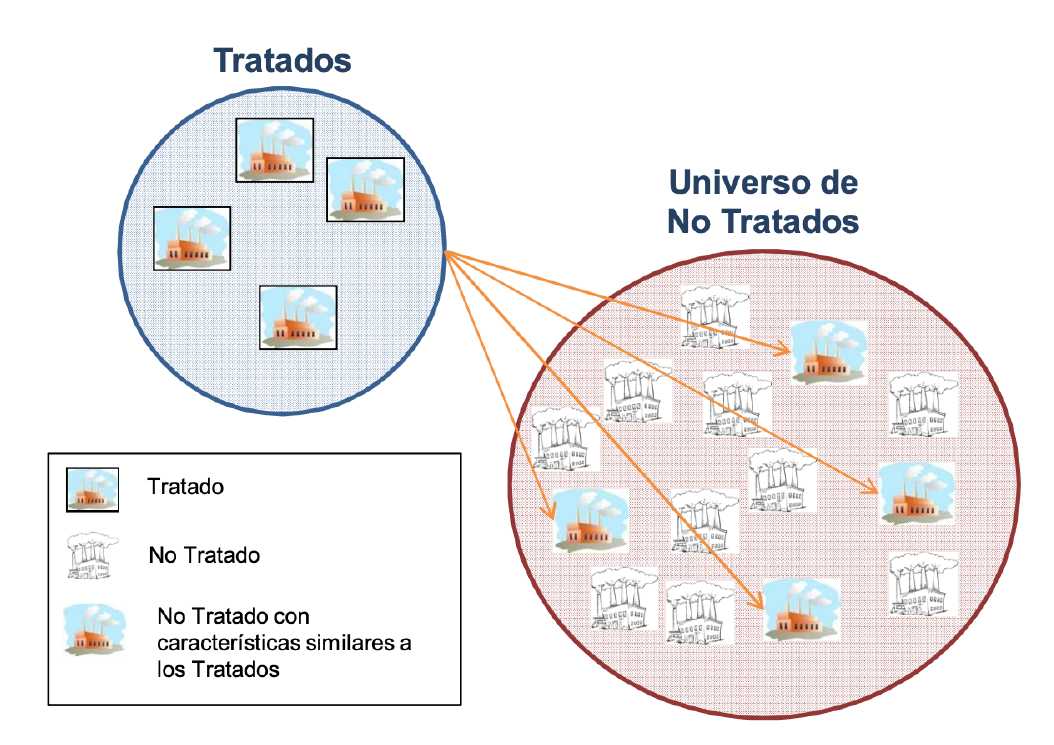
\includegraphics[width=0.65\textwidth]{figs/grupo-de-control.png}
    \caption{El grupo de control debería estar formado idealmente por individuos que no
    recibieron el tratamiento pero que en promedio poseen características similares a
    los tratados.}
    \label{fig:control-group}
\end{figure}

Por lo tanto, en la práctica, para obtener una buena estimación del \(ATT\), el reto está
en definir un \textit{buen} grupo de control, es decir uno que sea estadísticamente
idéntico al de tratamiento, en promedio, en ausencia del programa \cite{gertler-2016}. Si
se lograra que los dos grupos sean idénticos, con la única excepción que un grupo
participa del programa y el otro no, entonces sería posible estar seguros que cualquier
diferencia en los resultados tiene que deberse al programa \cite{gertler-2016}.

Para que un grupo de comparación sea válido, debe satisfacer lo siguiente \cite{gertler-2016}:
\begin{itemize}
    \item Las características \textit{promedio} del grupo de tratamiento y del grupo de
    comparación deben ser idénticas en ausencia del programa. Cabe resaltar que no es
    necesario que las unidades individuales en el grupo de tratamiento tengan clones
    perfectos en el grupo de control.
    \item No debe ser afectado por el tratamiento de forma directa ni indirecta.
    \item El grupo de comparación debería reaccionar de la misma manera que el grupo de
    tratamiento si fuera objeto del programa.
\end{itemize}
En general, no resulta sencillo verificar estos puntos, por lo que las técnicas de
evaluación que veremos a continuación suelen establecer algunos supuestos.

Cuando el grupo de comparación no produce una estimación precisa del contrafactual, no se
puede establecer el verdadero impacto del programa. A continuación, se presentan dos
situaciones comúnes en las que esto ocurre.

\subsubsection{Comparaciones antes-después}
Este tipo de comparaciones intenta establecer el impacto de un programa a partir de un
seguimiento de los cambios en los resultados en los participantes del programa a lo largo
del tiempo. Estiman el contrafactual con el resultado promedio para el grupo de
tratamiento antes que comience la intervención, momento también conocido como
\textbf{línea de base}. Si bien una ventaja de este método es que no es necesario hallar
un grupo de control, esta comparación supone que si el programa no hubiera existido,
el resultado para los participantes del programa habría sido igual a su situación antes
del mismo, lo cual en la mayoría de los tratamientos no puede sostenerse
\cite{gertler-2016}.

\subsubsection{Comparaciones de inscritos y no inscritos: Sesgo de autoselección}
Como explicamos anteriormente, el término \(\mathbb{E} \left[Y_i(0)|D_i=1\right]\) de la
Ecuación \ref{eq:ATT} representa el contrafactual, que no es observable. Sin embargo, lo
que sí se puede medir es la variable de resultado entre los no inscritos, aquellos
individuos que no participaron del programa, es decir \(\mathbb{E}
\left[Y_i(0)|D_i=0\right]\).

Por lo tanto, podríamos tomar a todo el conjunto de los no participantes como grupo de
control y solucionar el problema del contrafactual utilizando \(\mathbb{E}
\left[Y_i(0)|D_i=0\right]\) como estimador, es decir podríamos asumir lo siguiente:
\begin{equation}
    \mathbb{E} \left[Y_i(0)|D_i=1\right]\ = \mathbb{E} \left[Y_i(0)|D_i=0\right]\
    \label{eq:supuesto-1}  % IC: Independencia Condicional
\end{equation}
Esto quiere decir que el valor esperado de la variable de resultado en ausencia del
programa (\(\mathbb{E}\left[Y_i(0)\right]\)) es idéntico para el grupo de tratados (\(D_i =
1\)) y para el de no tratados (\(D_i = 0\)). Indica que los individuos que participan en el
programa no son sistemáticamente distintos de los que no lo hacen \cite{bernal} o, en
otras palabras, que la decisión de participar en el programa no está determinada por
factores que también influyen en la variable de resultado.

De esta forma, podríamos calcular el \(ATT\) como:
\begin{equation}
    ATT = \mathbb{E} \left[Y_i(1)|D_i=1\right] - \mathbb{E} \left[Y_i(0)|D_i=0\right]
    \label{eq:ATT-con-supuesto-IC}
\end{equation}

Sin embargo, el supuesto de la Ecuación \ref{eq:supuesto-1} se viola toda vez que la
participación en el programa es una \textit{elección} del individuo elegible
\cite{bernal}. La razón es que los participantes y los no participantes generalmente son
diferentes, aún en ausencia del programa, y son justamente esas diferencias que llevan a
que algunos individuos escojan participar y otros no. Por lo tanto, si en estos casos se
toma como grupo de control a todos aquellos que no decidieron participar y se mide el
impacto con respecto a ellos, puede ocurrir que la diferencia en los resultados se deba a
características propias de los individuos que llevaron a unos a anotarse y a otros no.

El problema descrito se conoce como \textbf{sesgo de autoselección}, ya que los
integrantes del grupo de control se \textit{autoseleccionaron} para no participar del
programa. Más concretamente, este sesgo se produce cuando los motivos por los que un
individuo participa en un programa, usualmente no observables y difíciles de medir, están
correlacionados con los resultados \cite{gertler-2016}, y por ende, es muy probable que la
variable de resultado del grupo de tratamiento y del grupo de control sea diferente,
\textit{aún si el programa no existiera} \cite{bernal}. Intuitivamente, si hay variables
que explican tanto la participación como el resultado potencial, la comparación de medias
puede estar atribuyendo al programa un efecto que en realidad se debe a las diferencias
preexistentes entre el grupo de tratamiento y el grupo de control \cite{bernal}.

Un buen ejemplo de esta situación lo presenta \cite{bernal}, en el que se plantea un
programa de nutrición infantil. Podría ocurrir por ejemplo que las madres de familias
participantes del programa sean más proactivas respecto al desarrollo de sus hijos, por lo
cual se preocuparon en lograr la participación en el programa. El problema de
autoselección en este caso radica en que la motivación de las madres (que no se observa y
es difícil de medir) afecta no solo la probabilidad de participar en el programa, sino
también el estado nutricional de los niños ya que estas podrían vigilar mejor la dieta de
sus hijos. De esta forma, la diferencia observada en el estado nutricional de los niños de
los dos grupos podría deberse parcialmente a la diferencia en el nivel de compromiso de
las madres, y no exclusivamente a que un grupo participa en el programa y el otro no.

Podemos plantear este problema más formalmente. Notemos que podemos reescribir la fórmula
del \(ATT\) (\ref{eq:ATT}) de la siguiente manera:
\begin{equation}
    ATT + \mathbb{E} \left[Y_i(0)|D_i=1\right] = \mathbb{E} \left[Y_i(1)|D_i=1\right]
    \label{eq:ATT2}
\end{equation}
Si ahora restamos \(\mathbb{E} \left[Y_i(0)|D_i=0\right]\) a ambos lados, obtenemos:
\begin{equation}
    ATT + \left( \mathbb{E} \left[Y_i(0)|D_i=1\right] - \mathbb{E} \left[Y_i(0)|D_i=0\right] \right) =
    \mathbb{E} \left[Y_i(1)|D_i=1\right] - \mathbb{E} \left[Y_i(0)|D_i=0\right]\
    \label{eq:ATT3}
\end{equation}

De esta forma, es claro que si los indivudos tratados son diferentes de los no tratados,
aún en ausencia del tratamiento (esto es \(\mathbb{E} \left[Y_i(0)|D_i=1\right] -
\mathbb{E} \left[Y_i(0)|D_i=0\right] \neq 0\)), entonces la diferencia entre sus medias
(el lado derecho de la igualdad) será igual al \(ATT\) más la diferencia preexistente
entre los grupos (el lado izquierdo de la igualdad) \cite{bernal}. Es decir, esta
comparación de medias será una combinación del efecto directo del tratamiento, capturado
en el \(ATT\), y las diferencias preexistentes y, sin información adicional, no es posible
distinguir qué parte se debe a qué \cite{bernal}.

Dicho esto, el gran desafío de la evaluación de impacto es determinar las condiciones o
supuestos bajo los cuales \(\mathbb{E} \left[Y_i(0)|D_i=0\right]\) se puede utilizar como
una estimación válida del contrafactual \(\mathbb{E} \left[Y_i(0)|D_i=1\right]\)
\cite{bernal}, y por lo tanto emplearse para poder aproximar el valor del \(ATT\).
Asegurarse de que el impacto estimado esté libre de sesgo de autoselección es uno de los
principales objetivos de cualquier evaluación de impacto, y plantea importantes
dificultades \cite{gertler-2016}.

\bigskip
Es importante en este punto identificar claramente las comparaciones que hemos
mencionado hasta el momento, los cuales se encuentran en la Tabla \ref{tab:distinciones}.
\begin{table}[h!]
    \centering
    \begin{tabular}{p{7cm}m{7cm}}  % Set fixed column widths
        \hline
        \textbf{Lo que se desea medir}: el \(ATT\). & \(\mathbb{E} \left[Y_i(1)-Y_i(0)|D_i=1\right]\) \\
        \hline
        \textbf{Lo que se observa}: el promedio de la diferencia entre los resultados de
        los tratados y el grupo de control. & \(\mathbb{E} \left[Y_i(1)|D_i=1\right]\) -
        \(\mathbb{E} \left[C_i(0)|D_i=0\right]\) \\
        \hline
        \textbf{El sesgo de autoselección}: las diferencias preexistentes entre el grupo de
        tratamiento y el de control. & \(\mathbb{E} \left[Y_i(0)-C_i(0)|D_i=0\right]\) \\
        \hline
    \end{tabular}
    \caption{Distinción entre las diferentes comparaciones presentes en una evaluación de impacto.}
    \label{tab:distinciones}
\end{table}

Teniendo en cuenta las fórmulas expuestas en la Tabla \ref{tab:distinciones}, podemos
enunciar de otra forma lo que dijimos anteriormente: la calidad de una evaluación de
impacto dependerá de los supuestos necesarios para asegurar que no hay sesgo de autoselección,
es decir que \(\mathbb{E} \left[Y_i(0)-C_i(0)|D_i=0\right] = 0\).

\bigskip
Las reglas de un programa para seleccionar a los participantes beneficiarios, también
llamadas \textbf{reglas de asignación}, constituyen un parámetro clave para determinar el
método de evaluación de impacto a utilizar para dicho tratamiento. A continuación,
presentamos las distintas reglas y los métodos de evaluación que se utilizan en la
práctica al trabajar con cada una de ellas.

\subsection{Evaluaciones Experimentales o Aleatorias}
Este tipo de evaluaciones se utiliza cuando los beneficiarios del programa en cuestión son
seleccionados de manera completamente aleatoria\footnotemark. Los tratamientos con esta
asignación son también llamados ensayos controlados aleatorios. \footnotetext{Cabe aclarar
que la asignación aleatoria se produce dentro de la población de unidades elegibles, que
está compuesta por aquellos individuos para los cuales interesa conocer el impacto del
programa \cite{gertler-2016}. Por ejemplo, si se está implementando un programa de
formación para los maestros de escuela primaria en zonas rurales, los maestros de escuela
primaria de zonas urbanas o los profesores de secundaria no formarían parte del conjunto
de unidades elegibles \cite{gertler-2016}.}

La asignación aleatoria trae dos consecuencias importantes: por un lado, las unidades ya
no pueden \textit{elegir} si participar o no, lo cual \textbf{elimina el sesgo de
autoselección}, y por el otro, todas tienen la misma probabilidad de ser seleccionadas
para el programa. De esta forma, el resultado potencial de cada individuo es independiente
de sus condiciones previas, ya que la asignación al tratamiento no está determinada por
sus características, sino por el azar. Esto hace que la asignación aleatoria sea el
métdodo más sólido para evaluar el impacto de un programa \cite{gertler-2016}.

Como explicamos anteriormente, el grupo de comparación ideal sería lo más similar posible
al grupo de tratamiento en todos los sentidos, excepto con respecto a su participación en
el programa que se evalúa. Ahora bien, el proceso de asignación aleatoria producirá dos
grupos que tienen una alta probabilidad de ser estadísticamente idénticos en todas sus
características (observables y no observables), siempre que el número de unidades sea
suficientemente grande \cite{gertler-2016}. Esto es así ya que en general, si esto ocurre,
este mecanismo asegura que cualquier rasgo de la población se transfiere a ambos grupos.
Sin embargo, en la práctica, este supuesto debería comprobarse empíricamente con los datos
de línea de base de ambos grupos.

Dicho esto, lo que sucede en estos casos es que todos aquellos individuos que no
resultaron ser beneficiarios del programa conforman un grupo de control que resulta ser
naturalmente un excelente estimador del contrafactual \(\mathbb{E}
\left[Y_i(0)|D_i=1\right]\). Es decir, mediante este tipo de asignación, se asegura que se
cumple el supuesto de la Ecuación \ref{eq:supuesto-1}.

Una vez que se haya asignado el tratamiento de manera aleatoria, gracias a la eliminación
del sesgo de autoselección y el consecuente cumplimiento de \ref{eq:supuesto-1}, es
bastante sencillo estimar el impacto del programa. Después que el programa ha funcionado
durante un tiempo, se miden los resultados de las unidades de tratamiento y de
comparación. El impacto del programa es sencillamente la diferencia entre el resultado
promedio para el grupo de tratamiento y el resultado promedio para el grupo de
comparación, es decir:
\[
    ATT = \mathbb{E} \left[Y_i(1)|D_i=1\right]\ - \mathbb{E} \left[Y_i(0)|D_i=0\right]\
\]

La asignación aleatoria puede utilizarse como regla de asignación de un programa en dos
escenarios específicos: cuando la población elegible es mayor que el número de plazas
disponibles del programa, o  cuando sea necesario ampliar un programa de manera progresiva
hasta que cubra a toda la población elegible \cite{gertler-2016}. Además, la asignación
aleatoria podría hacerse a nivel individual (por ejemplo, a nivel de hogares), o a nivel
de conglomerado (por ejemplo, comunidades) \cite{bernal}.

Resulta claro que las evaluaciones experimentales tienen varias ventajas: por diseño, al
quitarles la posibilidad de elección a los individuos sobre si participar o no en el
programa, resuelven el problema del sesgo de selección, y además los resultados obtenidos
son transparentes, intuitivos y no es necesario utilizar herramientas econométricas
sofisticadas para alcanzarlos \cite{bernal}. Esto hace que contribuyan a la transparencia
de las políticas públicas y a la rendición de cuentas \cite{bernal}.

Sin embargo, este tipo de experimentos sufre varias limitaciones que hace que no sea tan
común en la práctica. Por un lado, pueden ser costosos y de difícil implementación
\cite{bernal}. Esto se debe a que en general, el ensayo aleatorio se hace específicamente
para evaluar una intervención, por lo que es necesario destinar recursos para la prueba
piloto, la recolección de información, los seguimientos, y a veces incluso la
implementación del programa \cite{bernal}. Otro problema que tienen, y probablemente el
más importante, es que por pertenecer al grupo de control, se \textit{excluye} a un
segmento de la población, igualmente vulnerable y elegible, de los beneficios de la
intervención \cite{bernal}. Además, dada la imposibilidad de negar los beneficios a un
grupo de control por largos períodos, con frecuencia es imposible estimar los impactos de
largo plazo \cite{bernal}.

\subsection{Evaluaciones Cuasi-experimentales}
Cuando la asignación aleatoria de los participantes no es factible o plantea problemas
éticos, se emplean las llamadas evaluaciones o técnicas cuasi-experimentales, que son
aquellas que buscan estimar el impacto causal, pero a diferencia de las experimentales, no
se basan en la asignación aleatoria de la intervención \cite{gertler-2016}. En estos
casos, el programa que se intenta evaluar no tiene una regla de asignación clara que
explique por qué ciertos individuos se inscribieron en el programa y otros no lo hicieron,
por lo que se convierte en una incógnita adicional en la evaluación, acerca de la cual se
deben formular supuestos \cite{gertler-2016}. Para ello, estos métodos intentan
\textit{simular} la aleatorización de un diseño experimental controlando las diferencias
entre los individuos tratados y no tratados bajo diferentes hipótesis.

Si bien los métodos cuasi-experimentales suelen ser más adecuados en algunos contextos
operativos, su desventaja es que requieren más condiciones para garantizar que el grupo de
comparación provea una estimación válida del contrafactual, como veremos a continuación al
profundizar en algunos de ellos.

\subsubsection{Diferencias en Diferencias}
El modelo de diferencias-en-diferencias (DD) es una manera de controlar la estimación del
impacto por las diferencias preexistentes entre el grupo de tratamiento y el de control,
que estará formado por todos aquellos individuos elegibles que no recibieron el
tratamiento. Es decir, el DD no propone una forma de construir un grupo de control
adecuado sino una manera de aproximar el impacto que tenga en cuenta las diferencias entre
participantes y no participantes. A grandes rasgos, combina las comparaciones
antes-después con las comparaciones de inscritos y no inscritos, ambas discutidas
anteriormente.

Dada una variable de resultado \(Y\), este modelo establece el impacto como el cambio
esperado en \(Y\) entre el período posterior y el período anterior a la implementación del
tratamiento en el grupo de tratamiento, menos la diferencia esperada en \(Y\) en el grupo
de control en el mismo período \cite{bernal}. Es decir, \textbf{compara los cambios en los
resultados a lo largo del tiempo} entre unidades participantes y no participantes.

Si denotamos con \(Y^{(1)}\) al valor de la variable \(Y\) en la línea de base, es decir justo
antes de la implementación del programa, y con \(Y^{(2)}\) al valor de la misma variable en
un período posterior a la implementación (también llamado período de seguimiento),
entonces el impacto del programa por el método de DD está dado por\footnotemark
\footnotetext{Omitimos el subíndice \(i\) por comodidad}:
\begin{equation}
    ATT_{DD} =
        \left(
            \mathbb{E}\left[Y^{(2)}|D=1\right] - \mathbb{E}\left[Y^{(1)}|D=1\right]
        \right) -
        \left(
            \mathbb{E}\left[Y^{(2)}|D=0\right] - \mathbb{E}\left[Y^{(1)}|D=0\right]
        \right)
        \label{eq:dif-en-dif-1}
\end{equation}

Es importante señalar que el contrafactual que se estima en este caso es el cambio en los
resultados del grupo de tratamiento, y su estimación se logra midiendo el cambio en los
resultados del grupo de comparación \cite{gertler-2016}. En lugar de contrastar los
resultados entre los grupos de tratamiento y comparación después de la intervención, la
técnica de DD estudia las \textit{tendencias} entre los grupos de tratamiento y comparación
\cite{gertler-2016}.

Como explicamos con anterioridad, el principal problema de las comparaciones antes-después
en el grupo de tratamiento es que se asume que lo único que hizo cambiar la variable de
resultado fue el programa, cuando en realidad puede haber sido por factores externos. El
DD busca solucionar este problema basándose en la idea que la diferencia en los resultados
antes-después para el grupo de tratamiento controla por factores que son constantes a lo
largo del tiempo en ese grupo, y la manera de capturar los factores variables en el tiempo
es medir el cambio antes-después en los resultados de un grupo que no se inscribió en el
programa pero que estuvo expuesto al mismo conjunto de condiciones ambientales. De esta
forma, si se ``limpia'' la primera diferencia de otros factores variables en el tiempo que
influyen en el resultado de interés sustrayendo la segunda diferencia, se habrá eliminado
una fuente de sesgo \cite{gertler-2016}.

Por otro lado, en las comparaciones de inscritos y no inscritos, el gran inconveniente era
el sesgo de autoselección. Para entender mejor la solución que el DD propone a esto,
resulta conveniente reescribir el estimador como:
\begin{equation}
    ATT_{DD} =
        \left(
            \mathbb{E}\left[Y^{(2)}|D=1\right] - \mathbb{E}\left[Y^{(2)}|D=0\right]
        \right) -
        \left(
            \mathbb{E}\left[Y^{(1)}|D=1\right] - \mathbb{E}\left[Y^{(1)}|D=0\right]
        \right)
        \label{eq:dif-en-dif-2}
\end{equation}

De la Ecuación \ref{eq:dif-en-dif-2} se puede ver que lo que plantea es restarle al cambio
visto en la variable entre tratados y no tratados luego de la implementación del programa
(\(Y^{(2)}\)), las diferencias que ya pueda haber habido entre ellos en la línea de base
(\(Y^{(1)}\)). Es decir, desde este punto de vista, se utiliza a
\(\mathbb{E}\left[Y^{(1)}|D=1\right] - \mathbb{E}\left[Y^{(1)}|D=0\right]\) como un
estimador de las diferencias preexistentes entre el grupo de tratamiento y el grupo de
control.

Ahora bien, volviendo a la Ecuación \ref{eq:dif-en-dif-1}, el supuesto que permite
utilizar la diferencia en el grupo de no inscritos para controlar los factores externos
que afectan a los inscritos es que, en ausencia del programa, dichos factores habrían
impactado a los tratados de la misma manera que a los no tratados. En otras palabras, se
asume que, sin la intervención, los resultados en el grupo tratado habrían evolucionado en
paralelo con los del grupo de control, aumentando o disminuyendo en la misma proporción.
Esto se conoce como \textbf{supuesto de tendencias paralelas}, y es sobre el que hay que
basarse al trabajar con este método ya que claramente no es posible observar qué habría
ocurrido con el grupo tratado en ausencia del programa.

\subsubsection{Propensity Score Matching}
Otro enfoque para lograr una buena aproximación del contrafactual consiste en construir un
grupo de comparación artificial, a partir del conjunto de individuos que no recibieron el
tratamiento. En esto se basa el método conocido como \textbf{pareamiento} o
\textbf{emparejamiento}, que utiliza técnicas estadísticas y grandes bases de datos para
construir el mejor grupo de comparación posible sobre la base de características
observables \cite{gertler-2016}. La principal utilidad de este método es que puede
aplicarse en el contexto de casi todas las reglas de asignación de un programa, siempre
que se cuente con un grupo que no haya participado en el mismo \cite{gertler-2016}.

El supuesto que utilizan estas técnicas para basarse en características observables al
construir el grupo de control es que tanto la participación en el programa como los
resultados potenciales están únicamente determinados por estas. O, en otras palabras, que
no están determinados por variables no observables (o no medidas).

De esta forma, se asume que al condicionar los resultados potenciales de tratados y no
tratados en determinadas características observables (pertinentes en el programa bajo
estudio), el sesgo de autoselección es igual a cero. Formalmente, si denotamos con \(X\) a
los rasgos observables que se están teniendo en cuenta, este supuesto se escribe de la
siguiente forma\footnotemark :
\footnotetext{Nuevamente, omitimos el subíndice \(i\) por comodidad.}
\begin{equation}
    \mathbb{E}\left[Y(0)|D=1, X\right] = \mathbb{E}\left[Y(0)|D=0, X\right],
\end{equation}
y se lo conoce como \textbf{supuesto de Independencia Condicional} (IC).

Con esto en mente, la versión más directa de esta metodología consiste en encontrar un
``clon'' \textit{para cada individuo tratado} en el grupo de no tratados y contrastar las
variables de resultado de ambos \cite{bernal}. Un clon en este caso quiere decir, una vez
fijadas las características que el investigador cree que explican la decisión de
inscribirse en el programa, un individuo (o grupo de individuos) con exactamente las
mismas características observables \(X\).

Sin embargo, como mencionamos anteriormente, en la práctica esto resulta difícil. Si la
lista de características observables relevantes es muy grande, o si cada característica
adopta muchos valores, puede resultar computacionalmente complejo identificar una pareja
para cada una de las unidades del grupo de tratamiento. Esta situación es conocida como
\textit{el problema de la dimensionalidad}.

Para solucionarlo, se utiliza un método denominado \textbf{Pareamiento por Puntajes de
Propensión} (\textit{Propensity Score Matching}, PSM), presentado por primera vez en 1983
en \cite{psm1983}. Consiste en emparejar individuos pero no con base en \(X\), sino en su
probabilidad estimada de participación en el programa, dadas sus características
observables, es decir en:
\[P(X) = P(D = 1|X)\] donde \(P\) denota el operador de probabilidad de un evento . Este
valor es conocido como \textbf{probabilidad de participación} o \textbf{puntaje de
propensión}.

De esta forma, el clon adecuado para cada individuo del grupo de tratamiento
será aquel del grupo de no tratados con una probabilidad de participación en el programa
suficientemente cercana \cite{bernal}. La ventaja de emparejar a partir de \(P(X)\), a
diferencia de \(X\), es que \(P(X)\) es un número, mientras que \(X\) puede tener una
dimensión muy grande \cite{bernal}. Cabe aclarar que para calcular este puntaje, solo
deberían utilizarse las características en la línea de base, ya que post-tratamiento,
estas pueden haberse visto afectadas por el propio programa \cite{gertler-2016}.

Ahora bien, puede surgir la siguiente pregunta: ¿es posible encontrar (al menos) una pareja
para todos los individuos tratados? Y la respuesta es no, y para aquellos individuos no
será posible estimar el impacto del programa. Lo que puede ocurrir en la práctica es que
para algunas unidades inscritas, no haya unidades en el conjunto de no inscritos que
tengan puntajes de propensión similares. En términos técnicos, puede que se produzca una
falta de \textbf{rango o soporte común}.

La condición de soporte común (SC) establece que individuos con el mismo vector de
variables \(X\) tienen probabilidad positiva de ser tanto participantes como no
participantes del programa \cite{bernal}. Esto es, fijado un vector de variables
\(\hat{X}\):
\[0 < P(D=1|\hat{X}) < 1\] Si esta condición no se cumple, sería posible encontrar una
combinación particular de características que predice perfectamente la participación en el
programa, y por tanto, no existiría un individuo que fuera un buen control (o viceversa)
\cite{bernal}. Es decir, si por ejemplo para un vector de variables \(\hat{X}\), tenemos
que \(P(D=1|\hat{X})=1\), (o \(\simeq 1\)), entonces no podremos encontrar ningún no
tratado con esas características, y consecuentemente ningún control.

El SC implica que solo se utilizarán en la estimación aquellos individuos tratados para
los cuales se pueda encontrar uno no tratado con un puntaje de propensión similar. Por
ejemplo, si existen individuos del grupo de tratamiento con una probabilidad de
participación muy alta, pero ningún individuo no participante exhibe un puntaje tan alto,
entonces estos individuos tratados se descartarán a la hora de hacer el emparejamiento.

La Figura \ref{fig:common-support} muestra un gráfico de densidad de los puntajes de
propensión del grupo de tratados y del grupo de no tratados (suponiendo que ya se han
calculado en base a un determinado conjunto de características), en donde se puede ver que
hay falta de rango común. Lo que se hace en estos casos es simplemente restringir el
análisis a los individuos que se encuentran en el área de soporte común aunque esto, como
mencionaremos más adelante, puede traer problemas.

\begin{figure}[h!]
    \centering
    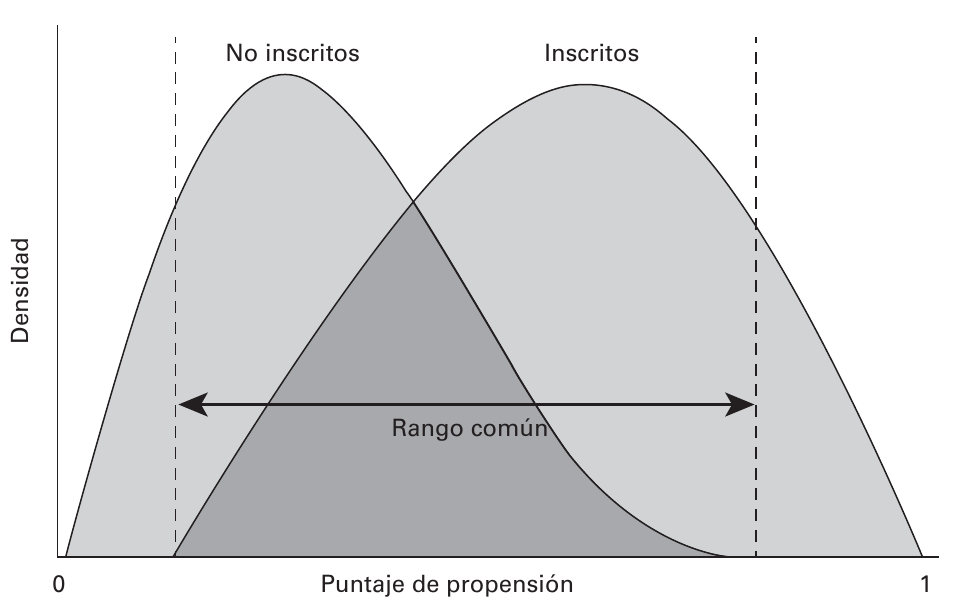
\includegraphics[width=0.65\textwidth]{figs/soporte-comun.png}
    \caption{Fuente: \cite{gertler-2016}. Gráfico de densidad de los puntajes de
    propensión de los tratados y los no tratados. El área entre las líneas punteadas es la
    región de soporte común, en donde se encuentran tanto inscritos como no inscritos con
    puntajes de propensión similares. En el área a la izquierda de dicha región solamente
    hay no inscritos con bajos puntajes de propensión. Es decir, lo que ocurre aquí es que
    \(P(D=1|\hat{X}) \simeq 0\). Similarmente, en el área a la derecha de la región de
    soporte común, solamente hay inscritos con altas probabilidades de participar. Es
    decir, lo que ocurre aquí es que \(P(D=1|\hat{X}) \simeq 1\), y para estos no será
    posible encontrar ningún individuo de control.}
    \label{fig:common-support}
\end{figure}

Asumiendo que se cumplen las condiciones de IC y SC, el estimador del \(ATT\) por PSM
estaría dado por:
\begin{equation}
ATT_{PSM} = \mathbb{E}_{P(X)|D=1}
    \left\{
        \mathbb{E}\left[Y(1)|D=1, P(X)\right] - \mathbb{E}\left[Y(0)|D=0, P(X)\right]
    \right\}
    \label{ATT-PSM}
\end{equation}
donde \(\mathbb{E}_{P(X)|D=1}\) es el valor esperado con respecto a la probabilidad de
participación \(P(X)\), condicional en ser participante del programa \cite{bernal}. Es
decir, un promedio ponderado de las diferencias entre llaves, donde los ponderadores
son funciones de la probabilidad de participación en el programa \cite{bernal}.

Los pasos a seguir a la hora de aplicar la técnica de PSM se pueden resumir en los
siguientes puntos:
\begin{enumerate}[label=\textbf{\arabic*.}]
    \item Identificar las unidades que se inscribieron en el programa y las que no lo
    hicieron.
    \item Definir el conjunto de variables observables \(X\) que se utilizarán para
    calcular el puntaje de propensión \(P(X)\).
    \item Calcular el puntaje de propensión \(P(X)\) para cada individuo, tratados
    y no tratados.
    \item Restringir la muestra al soporte común con respecto a la distribución
    del puntaje de propensión.
    \item Seleccionar un algoritmo de emparejamiento para emparejar a cada individuo
    tratado con un individuo o grupo de individuos no tratados que tenga una probabilidad
    de participación similar.
    \item Se calcula el impacto del programa como el promedio apropiadamente
    ponderado de la diferencia entre la variable de resultado de los tratados y
    sus parejas no tratadas (Ecuación \ref{ATT-PSM}).
\end{enumerate}
A continuación, se explican brevemente algunos de estos pasos.

En cuanto a la elección de variables (paso \textbf{2}) que se incluirán para calcular el
puntaje de propensión, si bien es importante poder parear utilizando un gran número de
características, lo es más aún hacerlo sobre la base de aquellas que \textbf{determinan la
inscripción} \cite{gertler-2016}.  En términos estadísticos, estas características reciben
el nombre de \textbf{covariables}, \textbf{variables independientes} o \textbf{variables
explicativas}, y son justamente aquellas que posiblemente predicen el resultado bajo
estudio.

Cuanto más se comprenda acerca de los criterios utilizados para la selección de los
participantes, en mejores condiciones se estará de construir un buen grupo de covariables
\cite{gertler-2016}. Para tener una mejor comprensión, los investigadores se pueden guiar
por los modelos económicos que describen el fenómeno bajo estudio, investigaciones previas
y conocimiento del diseño institucional \cite{bernal}. Además, como dijimos anteriormente,
estas características deben ser medidas en la línea de base, y no una vez aplicado el
programa, ya que se pueden haber visto afectadas por el mismo.

Con respecto al cálculo del puntaje de propensión (paso \textbf{3}), la idea es
especificar un modelo \(P(D=1|X) = f(X)\), es decir, la probabiliad de participación como
una función que puede ser lineal o no lineal en las características observables de los
individuos, \(X\) \cite{bernal}. Con frecuencia se prefieren los modelos de regresión
logística (\textit{logit}) o de probabilidad (\textit{probit}) \cite{bernal}. En este
trabajo, utilizaremos la regresión logística, por lo que resulta conveniente saber de qué
se trata.

Una regresión es un método en el cual se propone una relación funcional entre una variable
dependiente y una o varias variables independientes, y luego se estiman los coeficientes o
parámetros correspondientes a dicha relación funcional \cite{giuliodori-2022}. En el caso
del PSM, la variable dependiente es la probabilidad de participación y las independientes,
aquellas que el investigador haya seleccionado en el paso \textbf{2}. Cuando lo que se
intenta estimar es justamente una probabilidad, una opción es emplear el modelo de
regresión logística, que establece como relación funcional la llamada función logística o
sigmoide:
\[
    f(z) = \frac{e^z}{1 + e^z}
\]
El gráfico de esta función se puede ver en la Figura \ref{fig:logit}, donde se observa que
siempre da como resultado un valor real en el rango [0,1].

En la regresión logística, se toma \(z = \beta_0 + \beta_1 x_1 + \beta_2 x_2 + \dots +
\beta_k x_k\), siendo \(x_j\) las variables independientes y \(\beta_j\) los coeficientes
a estimar, correspondientes a la ponderación que tiene cada una de las variables. De esta
forma, suponiendo que se tienen dos clases o categorías ``0'' o ``1'', que en el PSM
serían respectivamente ``no participa'' y ``participa'', el valor dado por la función se
interpreta como la probabilidad que los valores de las variables independientes se
correspondan con la categoría 1, es decir: \(P(y=1|x_1, x_2, ..., x_k)\).

\begin{figure}[h!]
    \centering
    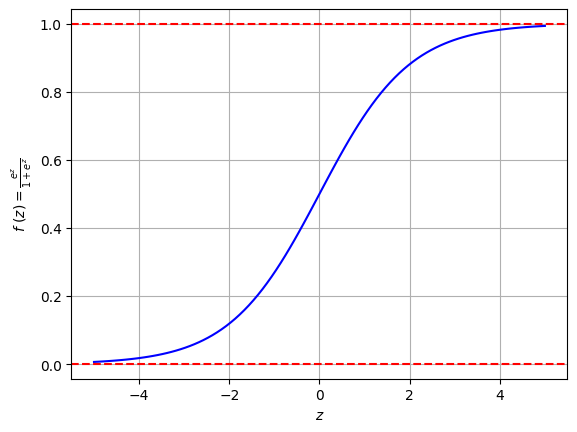
\includegraphics[width=0.65\textwidth]{figs/logit.png}
    \caption{Gráfico de la función logística para valores de \(z\) en el rango [-5,5].}
    \label{fig:logit}
\end{figure}

En lo que refiere al algoritmo de emparejamiento, estos suelen establecer tanto la manera
en que se encuentra el individuo (o grupo de individuos) ``parecido'' para cada tratado
como así también la manera en que se pondera la diferencia a la hora de hacer la
comparación. También se los llama estimadores ya que en fin, determinar una forma de
estimar el \(ATT\).

Uno de los más usados y más simples de entender es el de vecino más cercano (o \textit{NN
matching}, por su sigla en inglés, \textit{nearest neighbor}) \cite{bernal}. En el NN
matching, una opción es emparejar cada individuo de tratamiento con aquel del grupo de no
tratados que tenga la probabilidad de participación más cercana. Es decir, la unidad no
tratada tal que la distancia entre su puntaje y el del individuo tratado sea mínima. En
este caso, una vez que se haya emparejado a cada individuo tratado, el \(ATT\) se calcula
como el promedio simple de las diferencias entre las variables de resultado en cada
pareja.

Otra opción es dado un individuo tratado, tomar los \(k\) vecinos más cercanos del grupo
de no tratados con respecto al puntaje de propensión estimado, y estos formarán el grupo
de comparación para el tratado. Aquí, para calcular el impacto del programa, se puede dar
igual peso a cada uno de los \(k\) vecinos, en cuyo caso el impacto para una unidad
tratada estará dada por la diferencia entre la variable observada de ella y el promedio
simple de las variables de resultado de los vecinos cercanos \cite{bernal}. Otra
alternativa es hacer un promedio ponderado de las observaciones de los vecinos, según qué
tan comparable es cada vecino: así, el valor de la variable de resultado de un vecino más
cercano tiene más peso que el de uno no tan cercano.

Existen algunas cuestiones a tener en cuenta al utilizar este algoritmo, como puede ser
el hecho que la diferencia de puntajes entre un tratado y su vecino más cercano no
sea lo suficientemente pequeña como para asegurar que ambos son muy parecidos, y aún
así la diferencia entre sus variables de resultado contribuirá al cálculo del \(ATT\).

Otros algoritmos utilizados para el emparejamiento son los de \textit{kernel} y regresión
lineal local. Estos son estimadores no paramétricos que emparejan a cada individuo del
grupo de tratamiento con un promedio ponderado de (potencialmente) todos los individuos
del grupo de control \cite{bernal}. En principio, con estos, se puede comparar a cada
individuo de tratamiento con todos los no tratados, y darles menos peso en la comparación
a aquellos con probabilidades de participación más lejanas \cite{bernal}. Una ventaja de
ellos es que tienen menor varianza a la hora de calcular las diferencias individuales (que
vecino más cercano por ejemplo) porque usan más información \cite{bernal}. Para
más detalles sobre cada uno de estos, se puede consultar el Capítulo 6 de \cite{bernal}.

Una evaluación en la que se utilizó la técnica de PSM, particularmente con el algoritmo
del vecino más cercano, fue la llevada a cabo a partir del año 2021 por la Unidad de
Evaluación Integral de la Calidad y Equidad Educativa de la Ciudad Autónoma de Buenos
Aires (CABA) sobre el impacto del programa ``Jornada Extendida'' en el clima escolar
\cite{ueicee2023jornada}, aplicado sobre diferentes escuelas primarias de la ciudad. El
PSM fue empleado para seleccionar las escuelas del grupo de control en base a tres
características: el ISSAP (Índice de Situación Socioeconómica de los/as Alumnos/as en
Escuelas Primarias), la tasa de sobreedad y la tasa de repitencia.

Como mencionamos anteriormente, la gran ventaja del método de PSM es que es flexible,
pudiéndose utilizar en numerosos contextos, independientemente de la regla de asignación
de un programa, por lo que se emplea con frecuencia \cite{bernal}.

Sin embargo, es muy importante notar que los resultados arrojados por el PSM serán
confiables solamente si se cumple el supuesto de IC. Es decir, cuando existan razones para
pensar que las variables no observables o no disponibles en la base de datos no son un
determinante fundamental tanto de la participación en el programa como de las variables de
resultado potenciales. En otros términos, cuando no haya diferencias sistemáticas en las
características no observables entre las unidades tratadas y las de comparación pareadas
que puedan influir en el resultado.

Cabe aclarar que el supuesto de IC no puede ser demostrado, ya que no se puede verificar
si lo no observado afecta o no la decisión de participación, pero su plausibilidad puede
ser argumentada basándose en el conocimiento sustantivo del área de estudio. Otra
alternativa que se lleva a cabo en la práctica es calcular las diferencias en las
variables observables \(X\); si los dos grupos son demasiados diferentes en estas, esto
podría ser evidencia de que es probable que también existan diferencias entre los dos
grupos en características no observadas \cite{bernal}.

Por otro lado, si bien el cálculo del \(ATT\) se puede restringir a aquellos individuos
que se encuentra en la región de soporte común entre tratados y no tratados, esta
restricción puede volverse preocupante cuando hay una fracción importante de individuos
tratados que quedan sin emparejar. Esto implica que existirá un conjunto de individuos
para el cual no se puede decir nada acerca del efecto del programa \cite{bernal}.

\bigskip
En este trabajo, utilizaremos el PSM con el algoritmo de 1 vecino más cercano como
referencia para compararlo con nuestro enfoque, lo cual se explicará con más detalle en la
sección \ref{sec:problema}.

A continuación, introducimos el área de Inteligencia Artificial, dentro de la cual se
enmarcan los algoritmos propuestos en este trabajo.
\end{document}